\paragraph{Signatures including a Z boson}

\subparagraph{Z+\MET signature, leptonic channel}

The overall cross-sections in the \tanb and mass scans are shown in Fig.~\ref{fig:monoz_ll_xs_inclusive}.

\begin{figure}
\centering
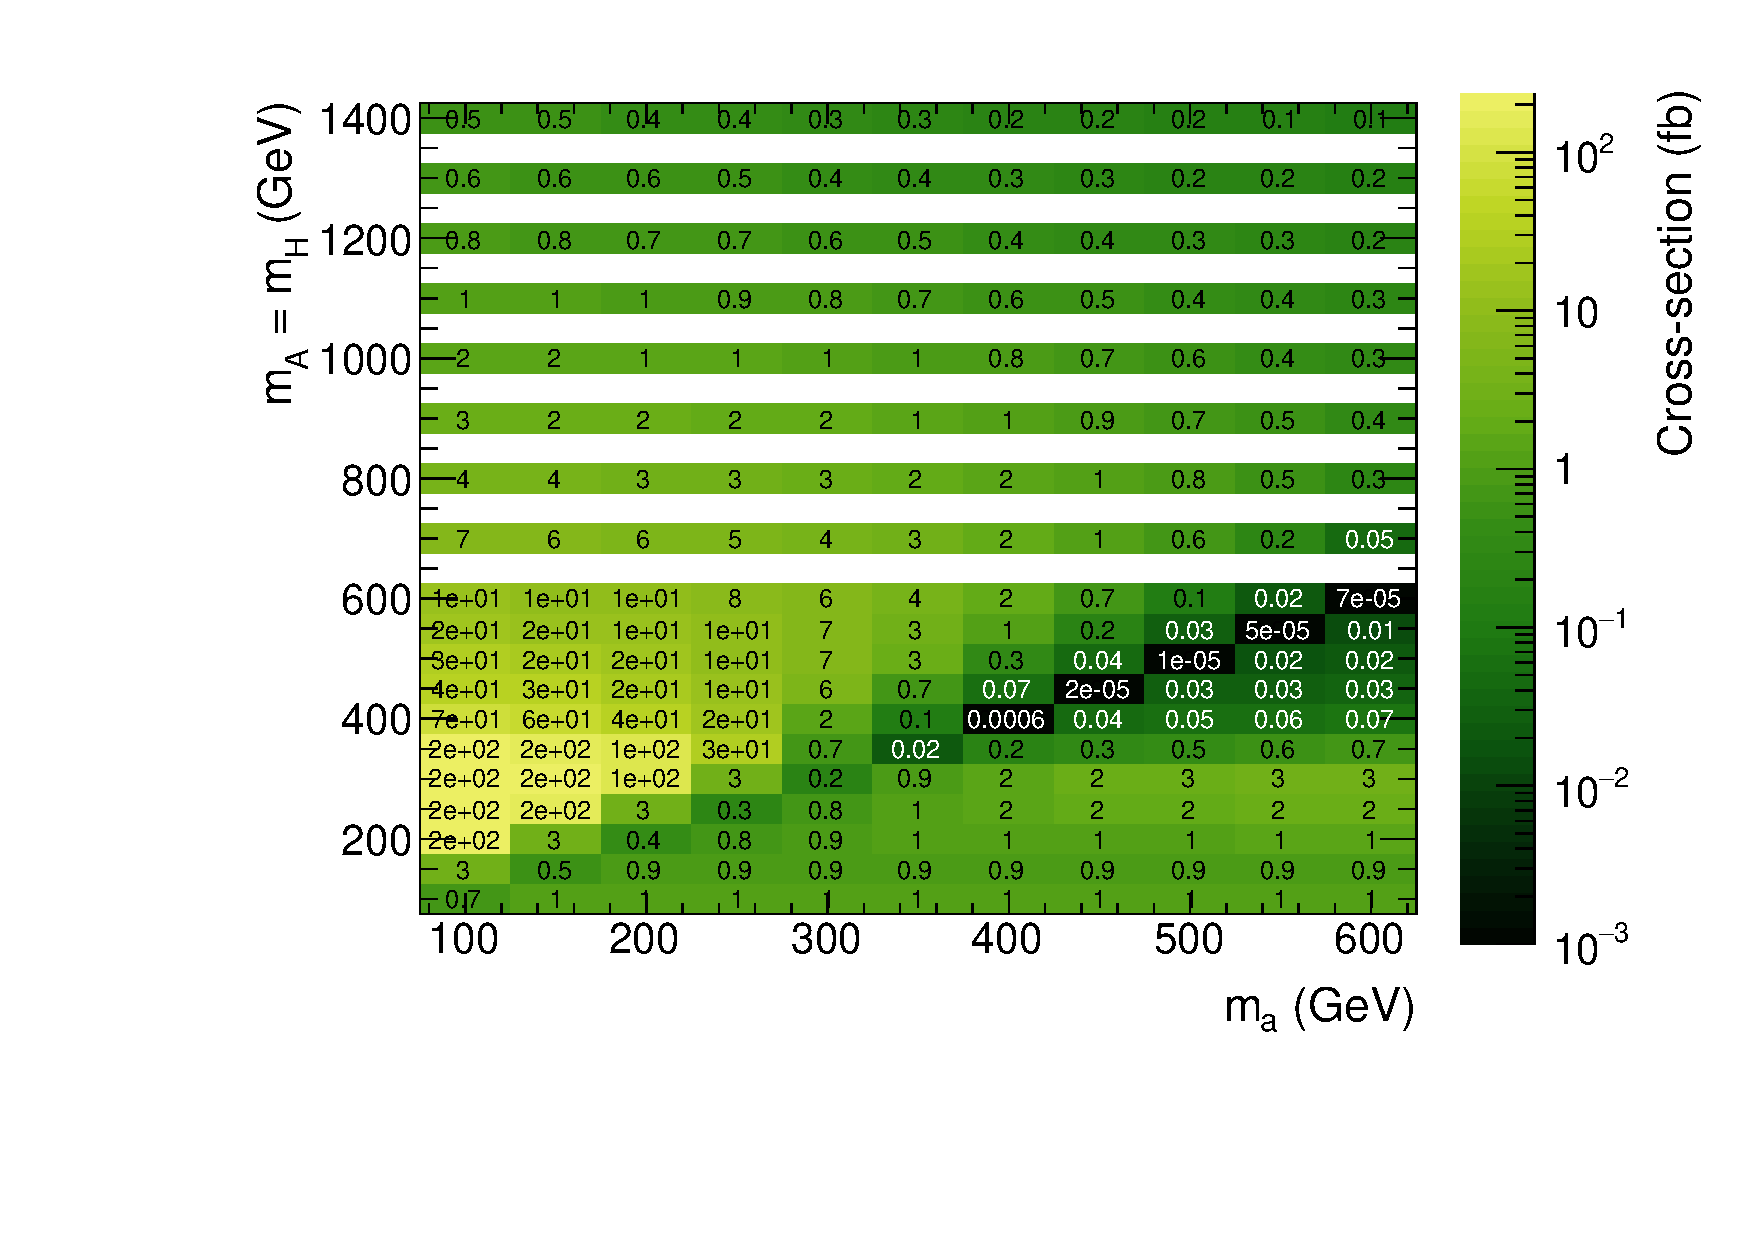
\includegraphics[width=0.8\textwidth]{texinputs/04_grid/figures/monoz/leptonic/xs_2d_inclusive_26300.pdf}
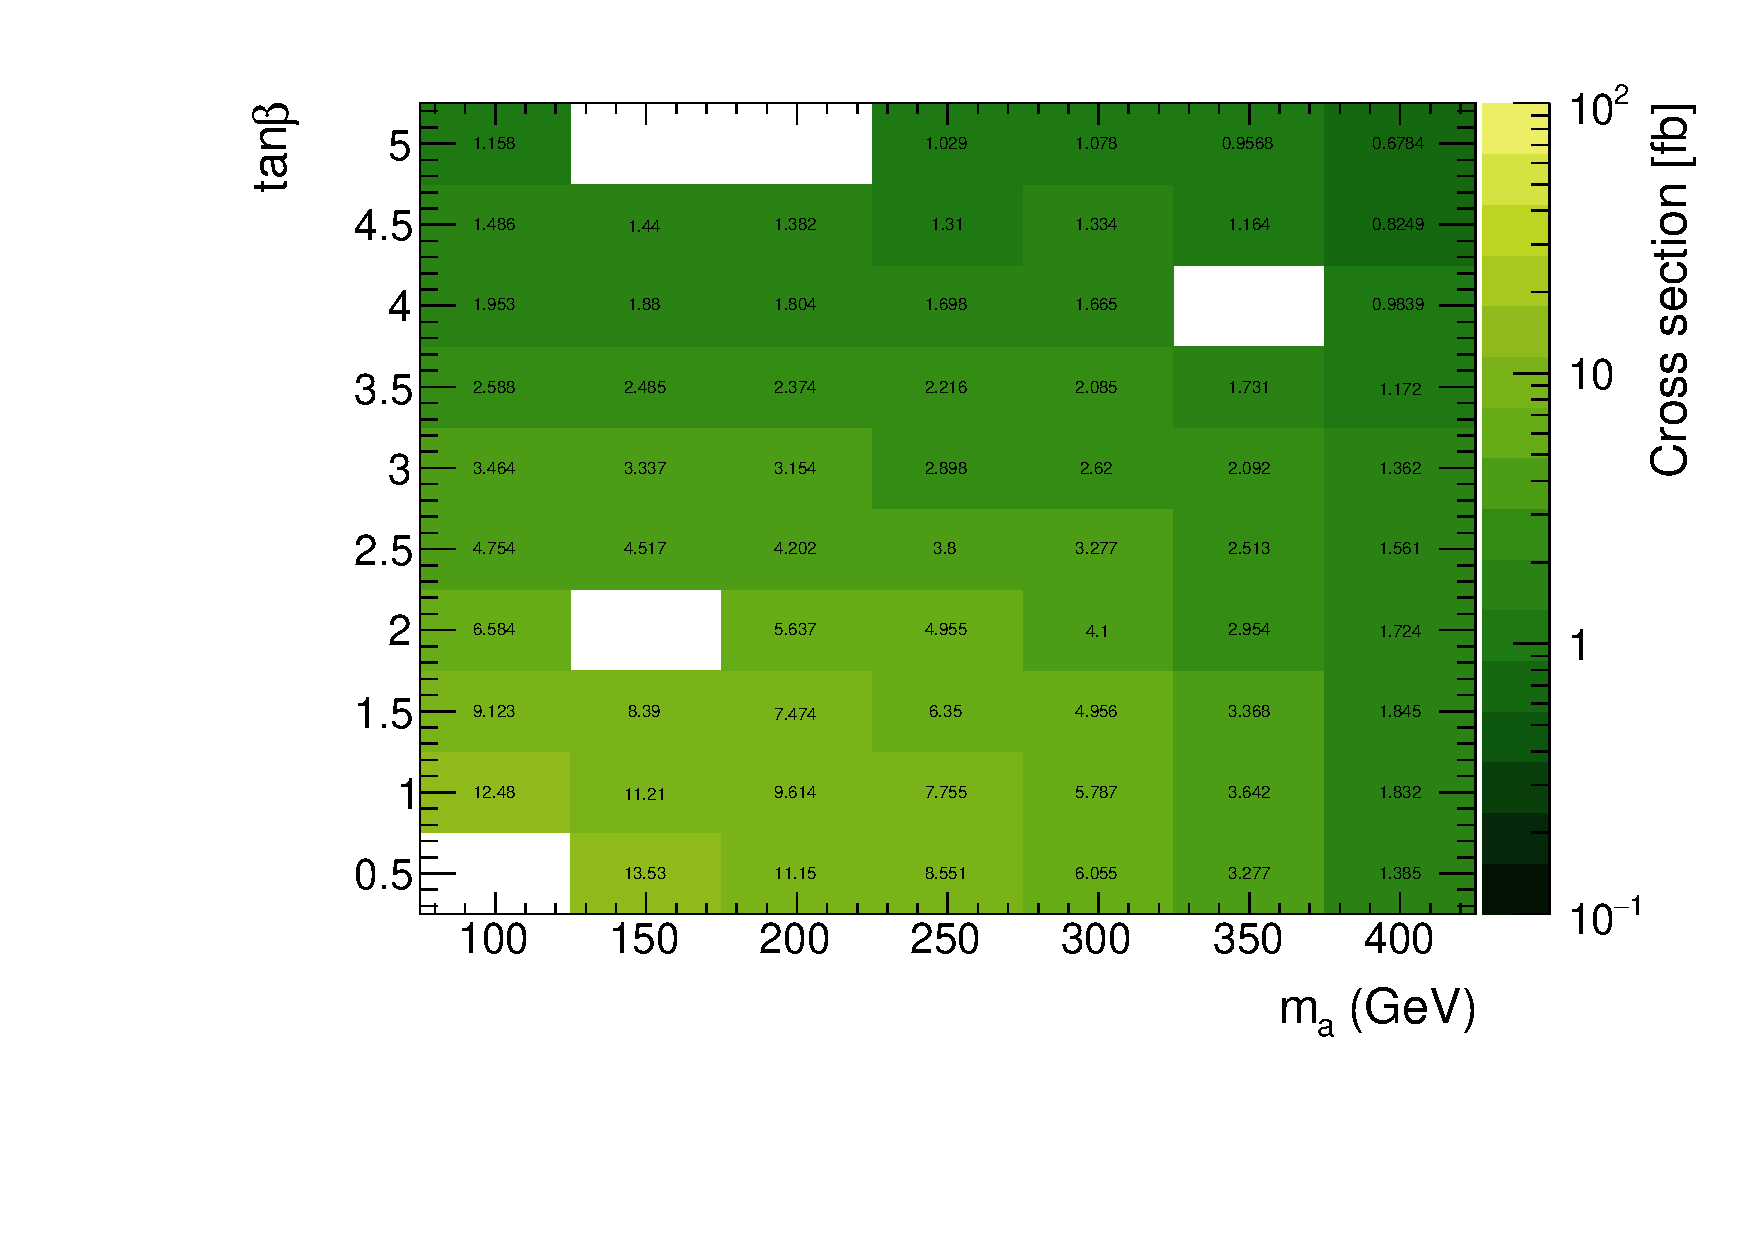
\includegraphics[width=0.8\textwidth]{texinputs/04_grid/figures/monoz/leptonic/tanbma_xsec_ll.pdf}
\caption{Inclusive cross-sections for $pp\rightarrow \lp\lm\chi\overline{\chi}$ in the \ma-\mA (top) and \ma-\tanb scans (bottom).}
\label{fig:monoz_ll_xs_inclusive}
\end{figure}

In the mass scan, maximal cross-sections are observed for the region of $\ma < \mA$ for values of $\ma\gtrsim100$ GeV. Towards higher values of both \ma and \mA, the cross-sections fall off, reaching values smaller than $1$ fb at $\ma\approx450$ GeV or $\mA\approx1.1$ TeV. In the $\ma\approx\mA$-region, the cross-section is suppressed by destructive interference. For the region with inverted mass hierarchy $\ma>\mA$, cross-sections of the order of multiple fb are observed, as long as $|\ma-\mA|$ remains sufficiently large.
In the \tanb scan, cross-sections smoothly fall with increasing $\ma$ as well as $\tanb$. Cross-sections are typically larger than 1 fb up to $\tanb\approx5$. The $\ma$ dependence is modulated by the value of \tanb: Crossing the $\ma$ range from $100$ to $400$ GeV, cross-sections are reduced by a factor $\approx7$ for small $\tanb\approx1$, but only a factor $\approx2$ for higher values of $\tanb\approx5$.
In the \sinp scan shown in Figure \ref{fig:monoz_ll_sinp_scan_xsec}, cross sections depends on whether or not the $a \rightarrow \ttbar$ decays are accesible.  
For $\ma < 350$ GeV they are not accesible and cross section strictly increases with \sinp.  For $\ma > 350 \GeV$, the $a \rightarrow \ttbar$ decays become possible causing the cross section to decrease for large values of \sinp.

%For \ma <350 GeV they are not accesible,  and only the heavy scalar's branching fraction to $aZ$ is relevant.  This branching fraction stricly increases with \sinp.  For \ma > 350 \GeV, the branching fraction of $a \rightarrow \chi \chi$ also becomes important, and there is a turnover point were the cross section decreases.

\begin{figure}
\centering
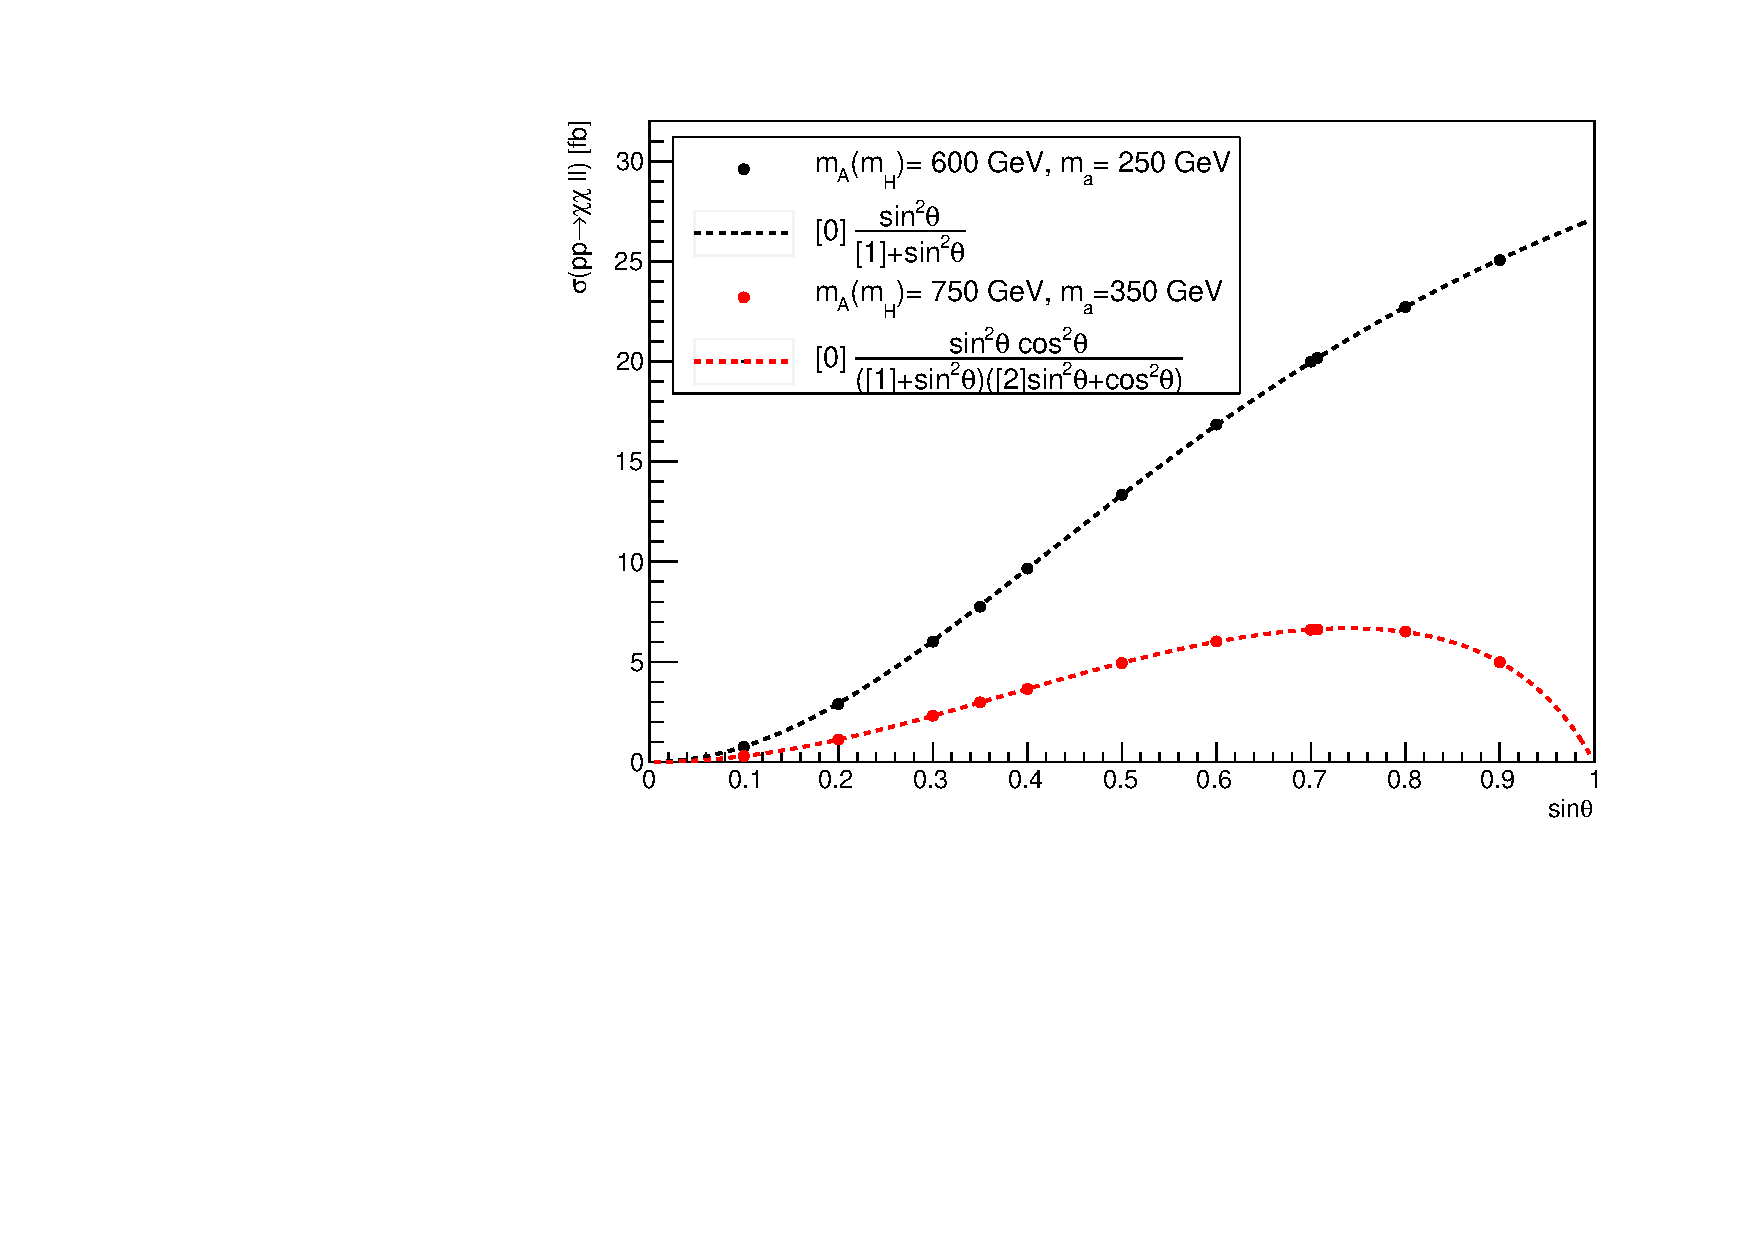
\includegraphics[width=0.6\textwidth]{texinputs/04_grid/figures/monoz/leptonic/SinThetaScan_xsecs.pdf}
\caption{For two different mass points, this figure shows the cross section $pp\rightarrow\chi\chi\ell\ell$ as a function of \sinp. 
For $\ma < 350$ GeV, $a$ decays solely to dark matter particles.  
As a consequence, the mixing angle only impacts the heavy scalar's branching fraction to $aZ$ and 
cross section strictly increases with \sinp.  
For \ma above 350 \GeV, \ttbar~ decays become accesible, introducing additional \sinp and \cosp dependences for the branching fraction 
of $a\rightarrow\chi\chi$.  For \ma above 350 GeV for large values of \sinp, there is a turnover point where the reduced $a\rightarrow\chi\chi$ branching fraction outweights the increased $H \rightarrow aZ$ branching and the net cross section decreases.}
\label{fig:monoz_ll_sinp_scan_xsec}
\end{figure}

\subparagraph{Z+\MET signature, hadronic channel}

\begin{figure}
\centering
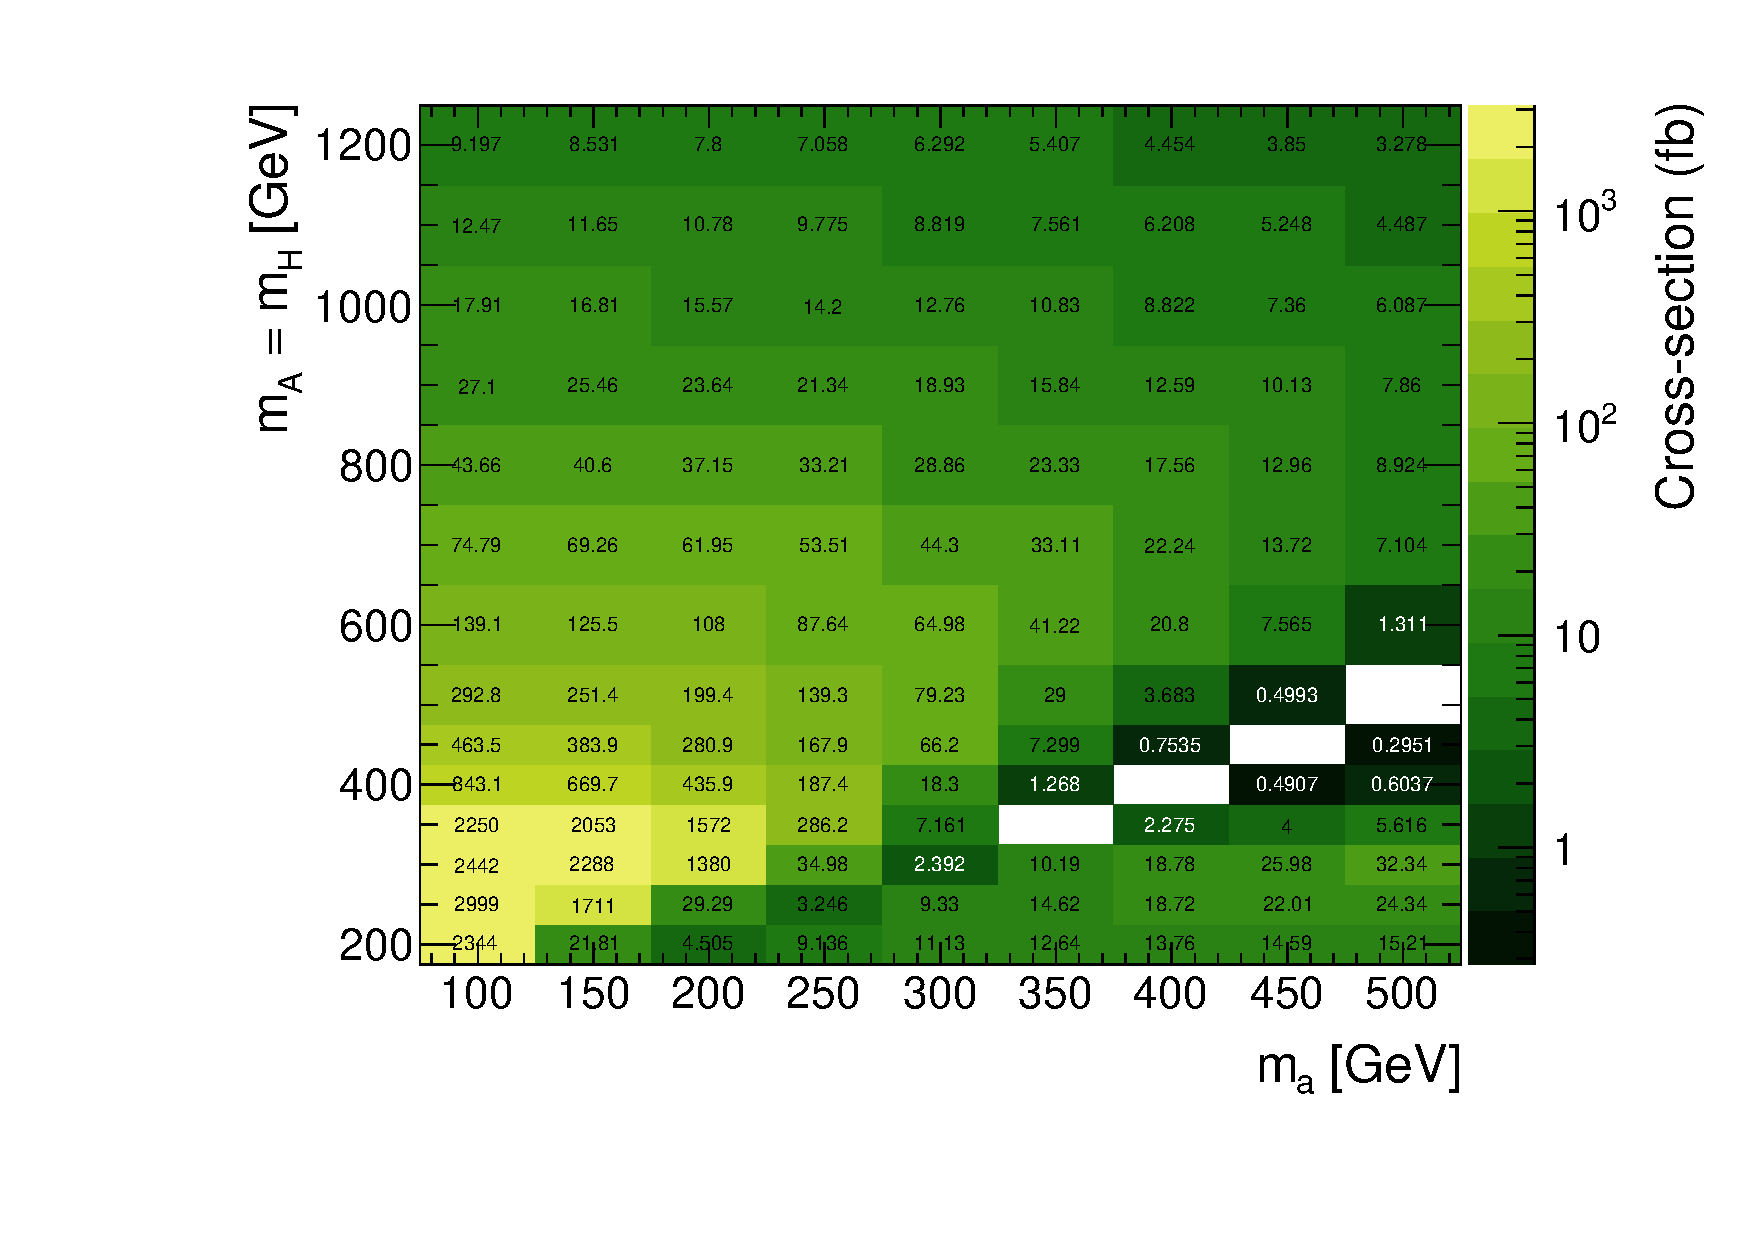
\includegraphics[width=0.45\textwidth]{texinputs/04_grid/figures/monoz/hadronic/grid_mA_ma_xsec.pdf}
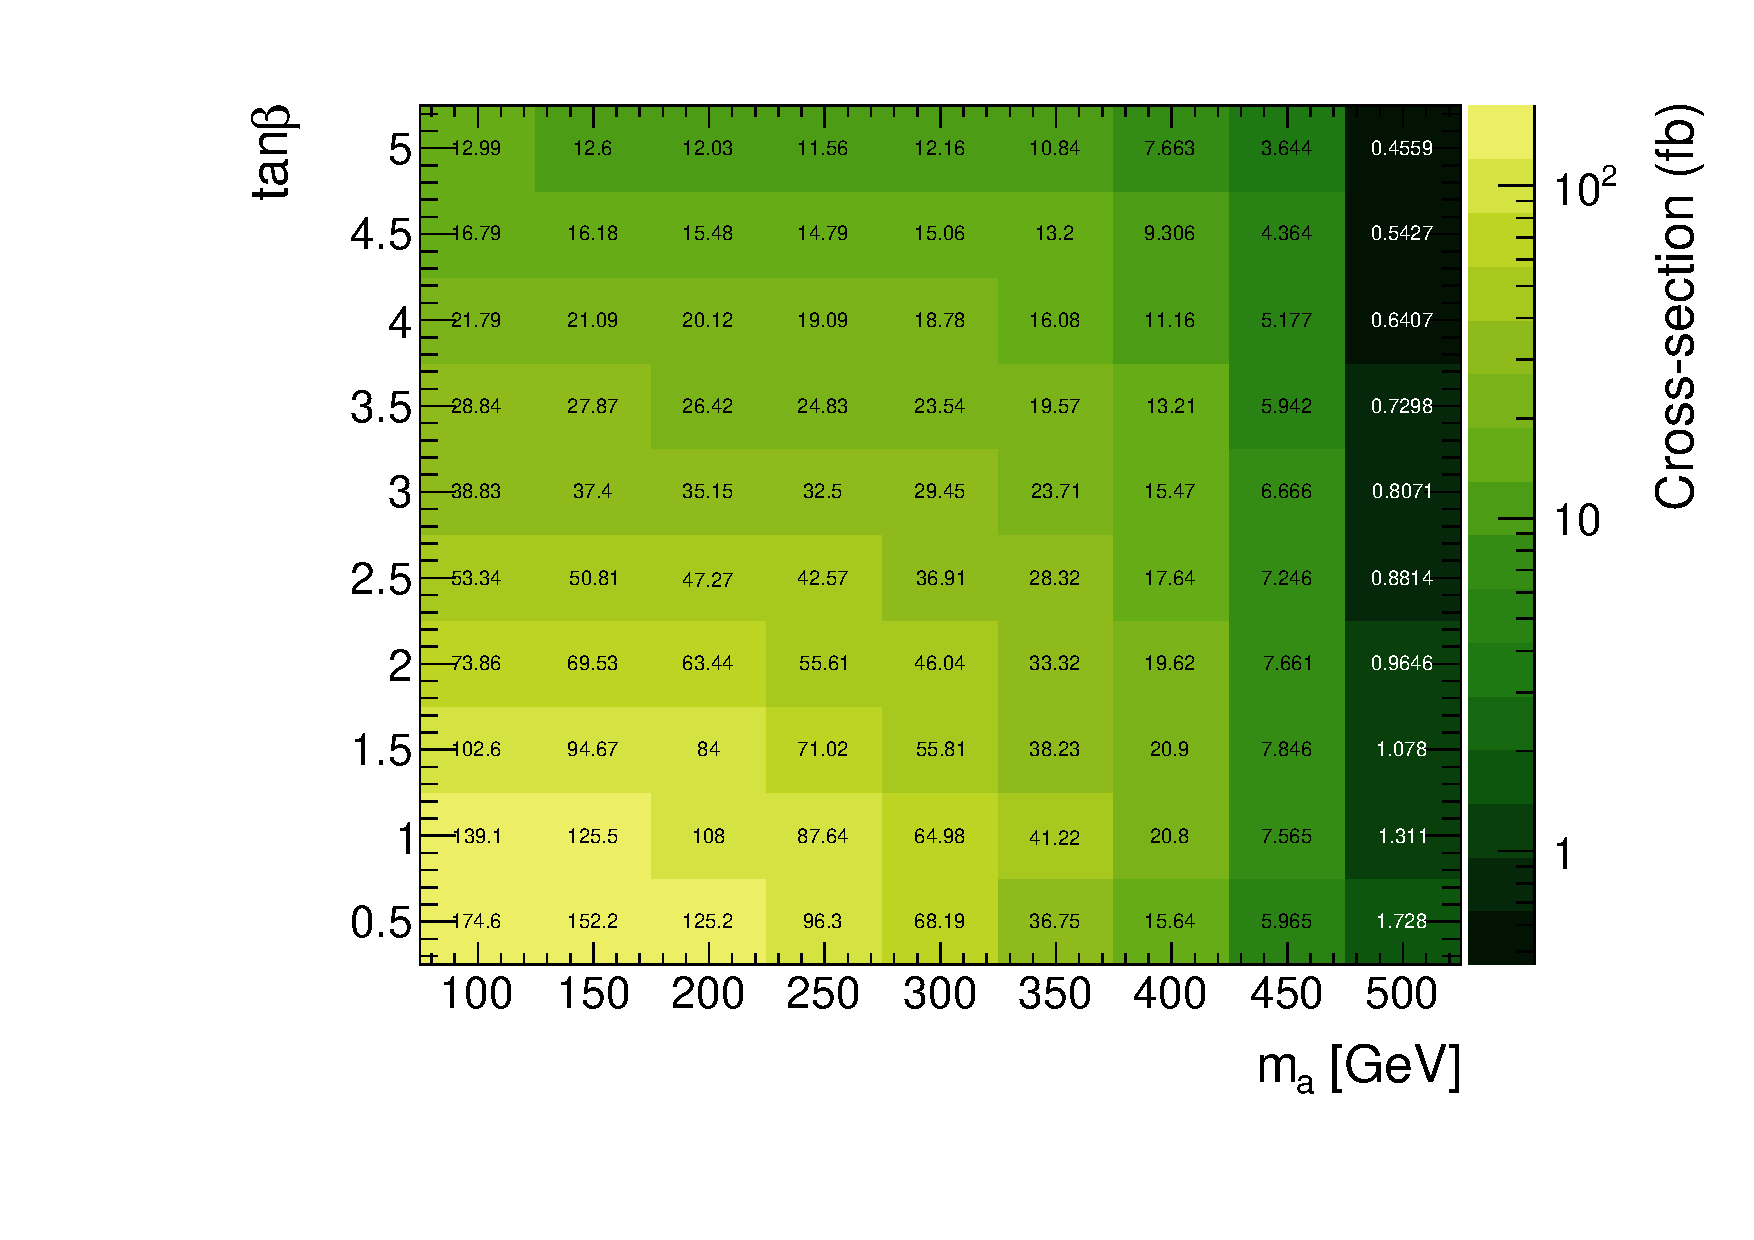
\includegraphics[width=0.45\textwidth]{texinputs/04_grid/figures/monoz/hadronic/grid_tanb_ma_xsec.pdf}
\caption{Inclusive cross-sections for the mono-$Z$ hadronic events 
$pp \rightarrow Z(\to q\bar{q})\chi\overline{\chi}$ in the \ma vs \mA (left) and \ma vs $\tan\beta$ (right) grids.
The $Z \to q\bar{q}$ branching fraction is not included in the cross-section.}
\label{fig:monozhad_inc_xsec_grid}
\end{figure}

Figure~\ref{fig:monozhad_inc_xsec_grid} shows the production cross-section for mono-$Z$ events 
in the $M_a$ ($M_A$) range between 100 and 500~GeV (200 and 1200~GeV). Shown on the left (right) is 
the cross-section in the \ma vs \mA (\ma vs $\tan\beta$) grid. Note that the $Z \to q\bar{q}$ branching fraction 
is not included in the cross-section. The production cross-section 
tends to vanish in the region where the $M_a$ gets close to $M_A$, as shown by the empty points in the grid.

\begin{figure}
\centering
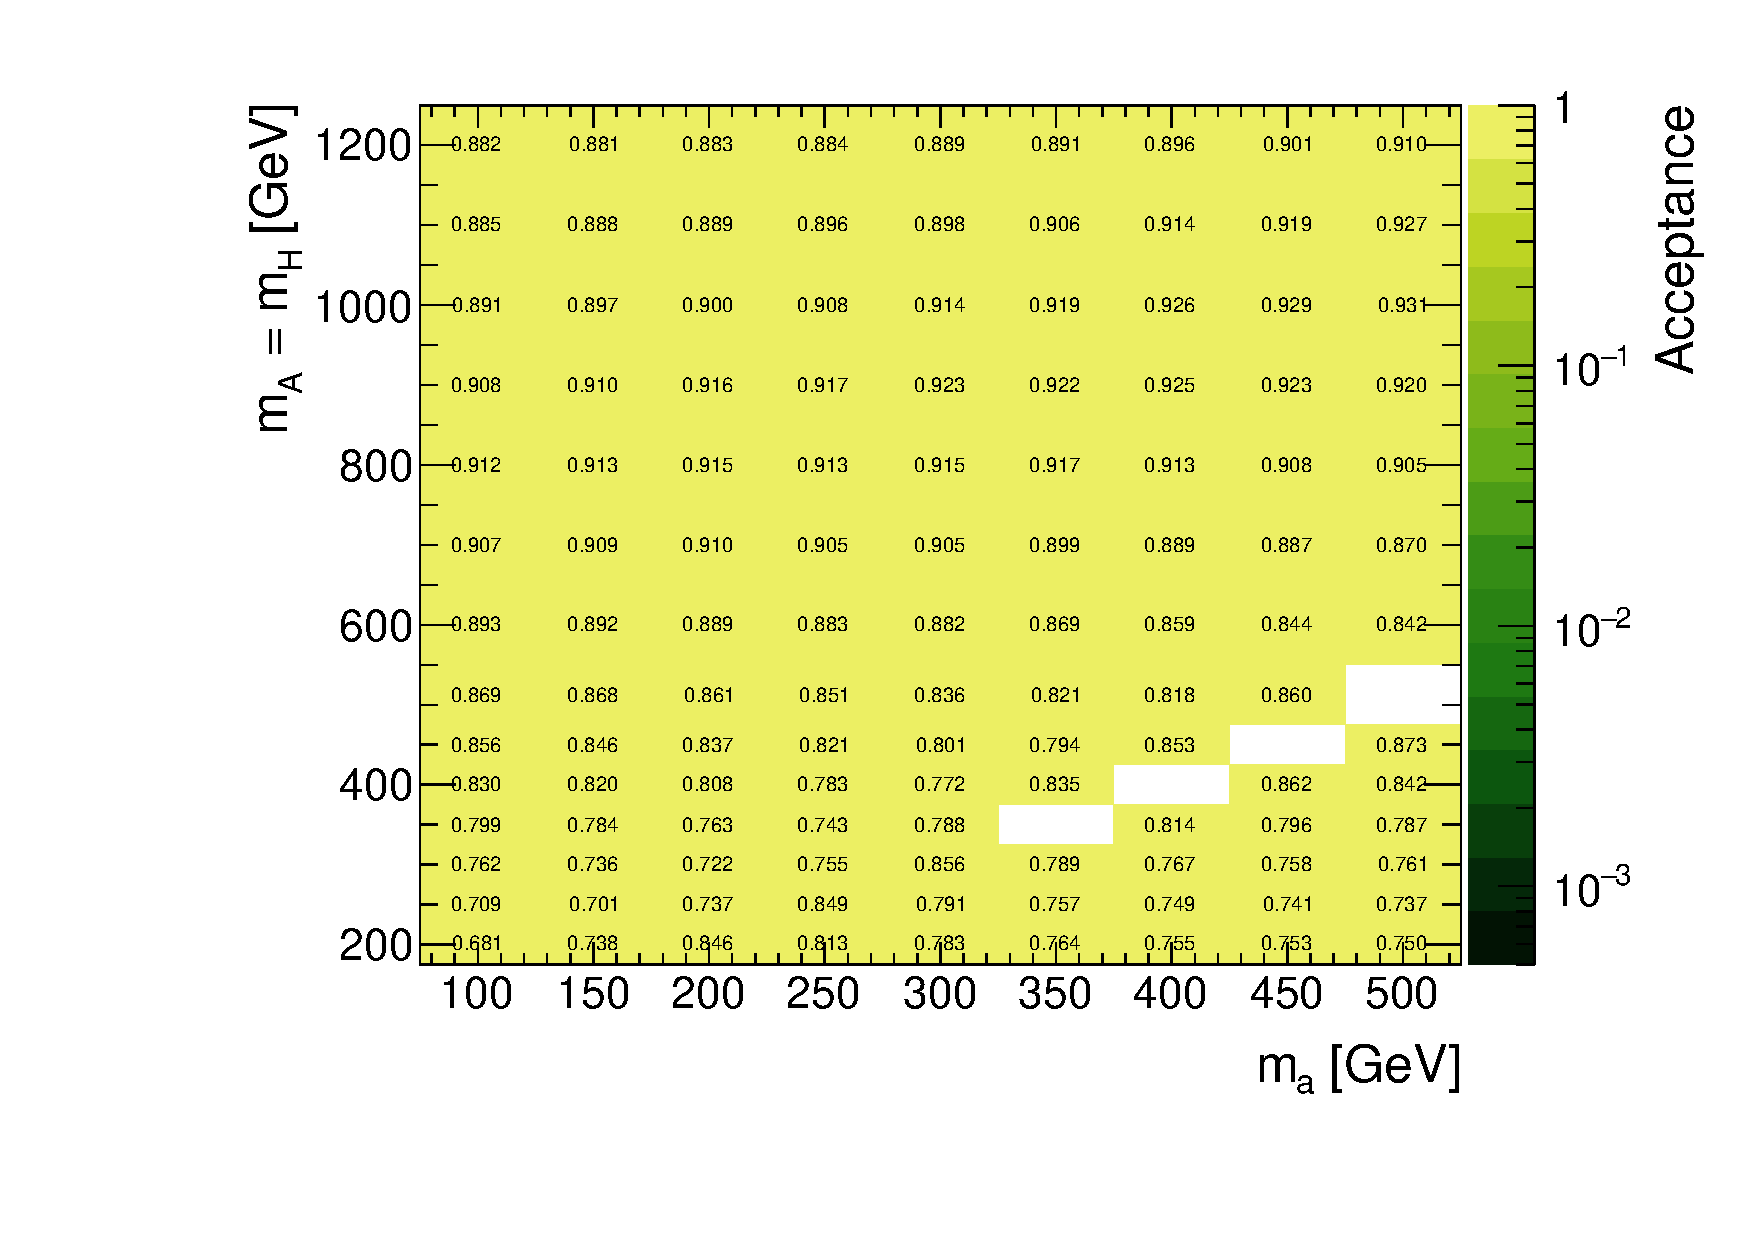
\includegraphics[width=0.45\textwidth]{texinputs/04_grid/figures/monoz/hadronic/grid_mA_ma_incl_resl_acc.pdf}
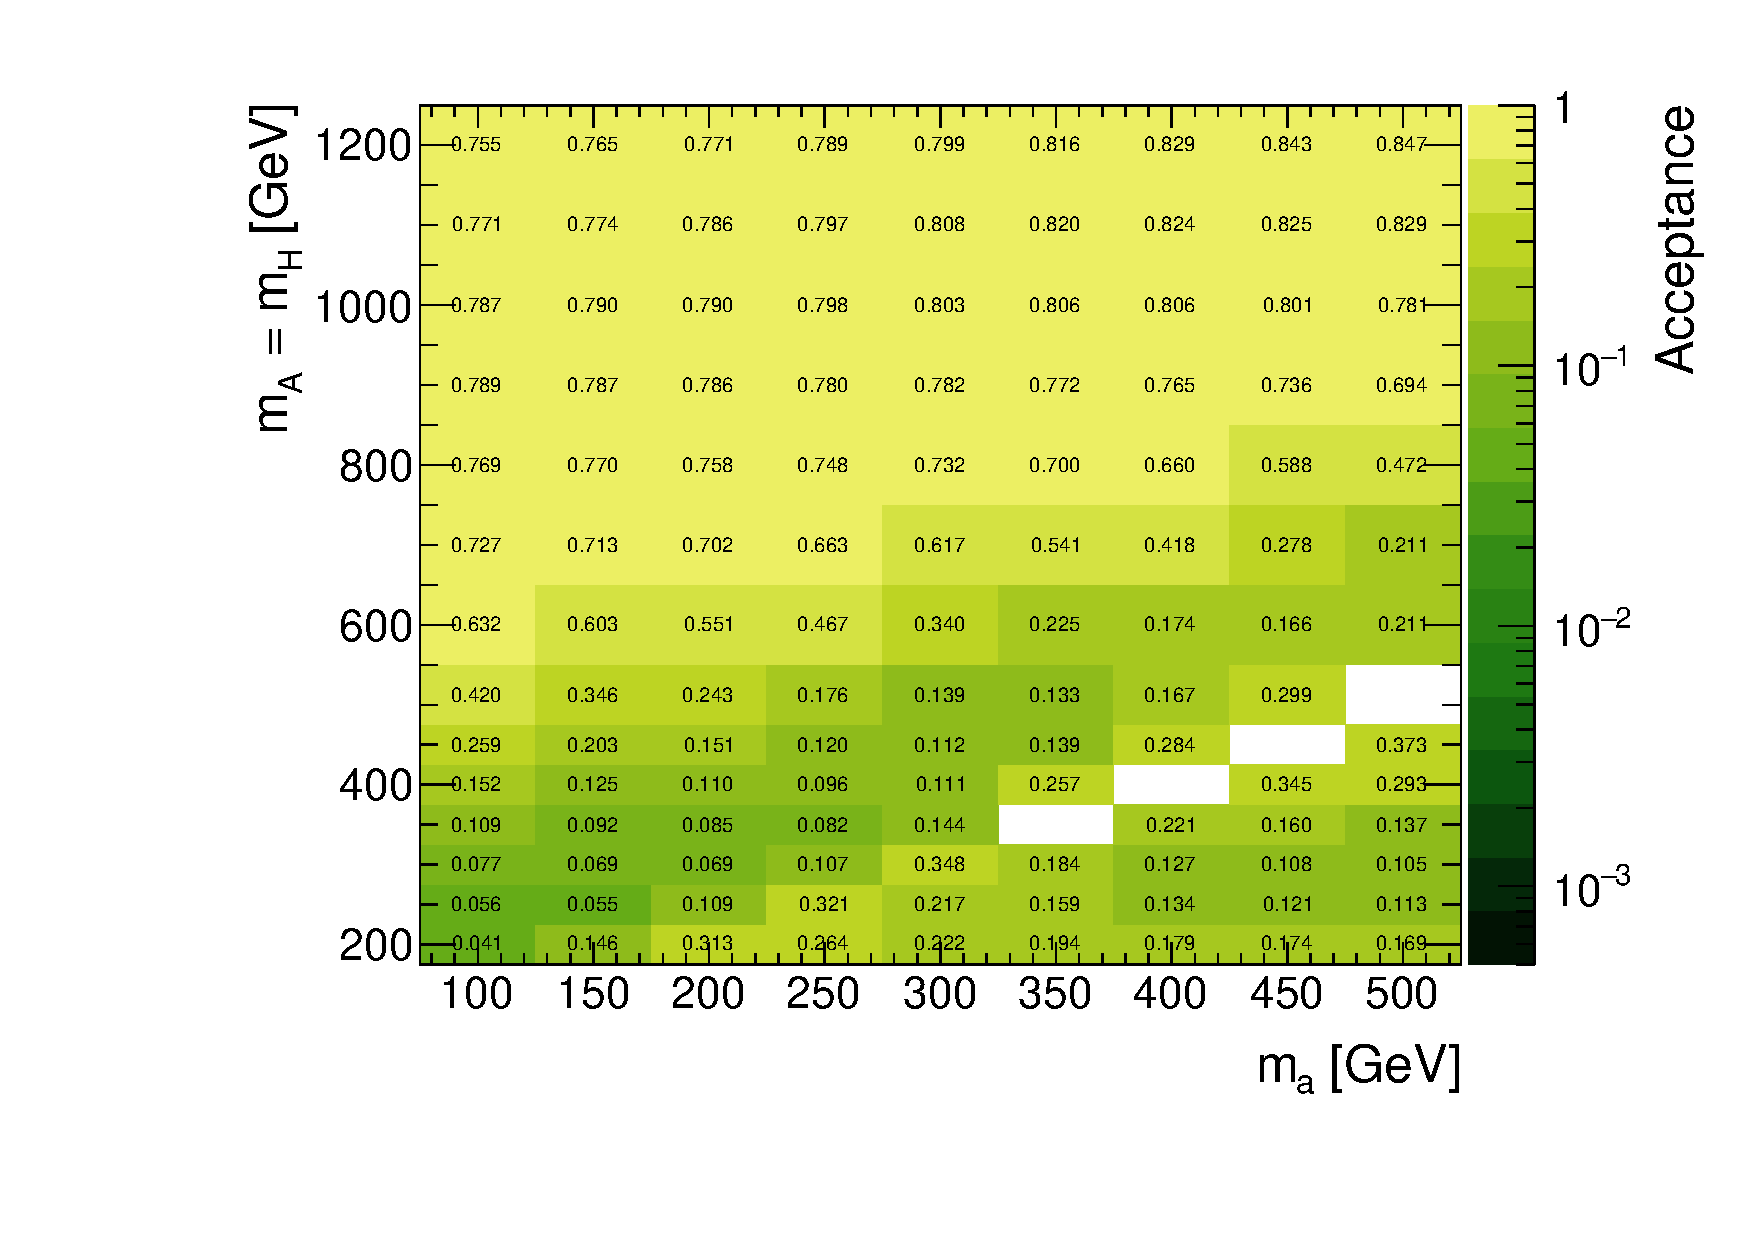
\includegraphics[width=0.45\textwidth]{texinputs/04_grid/figures/monoz/hadronic/grid_mA_ma_incl_merged_acc.pdf}
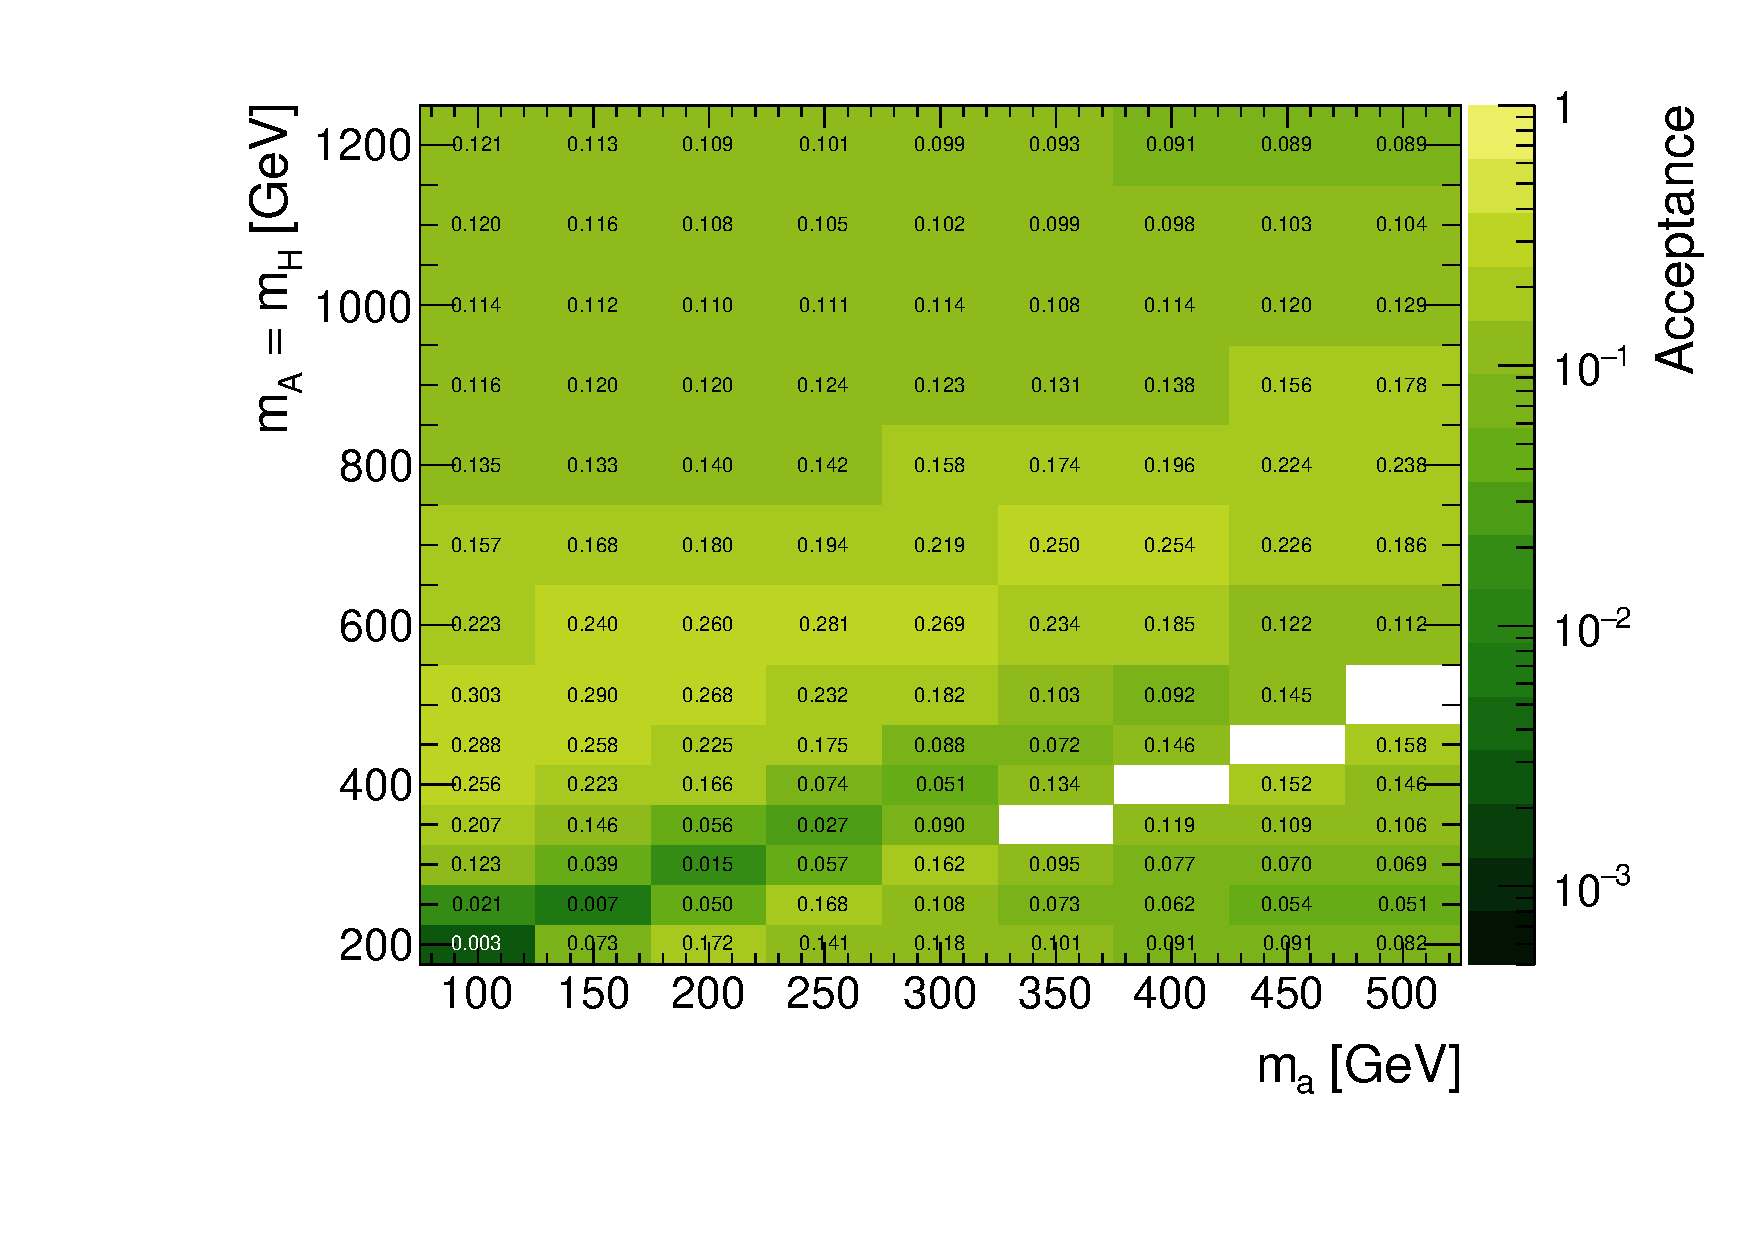
\includegraphics[width=0.45\textwidth]{texinputs/04_grid/figures/monoz/hadronic/grid_mA_ma_resl_acc.pdf}
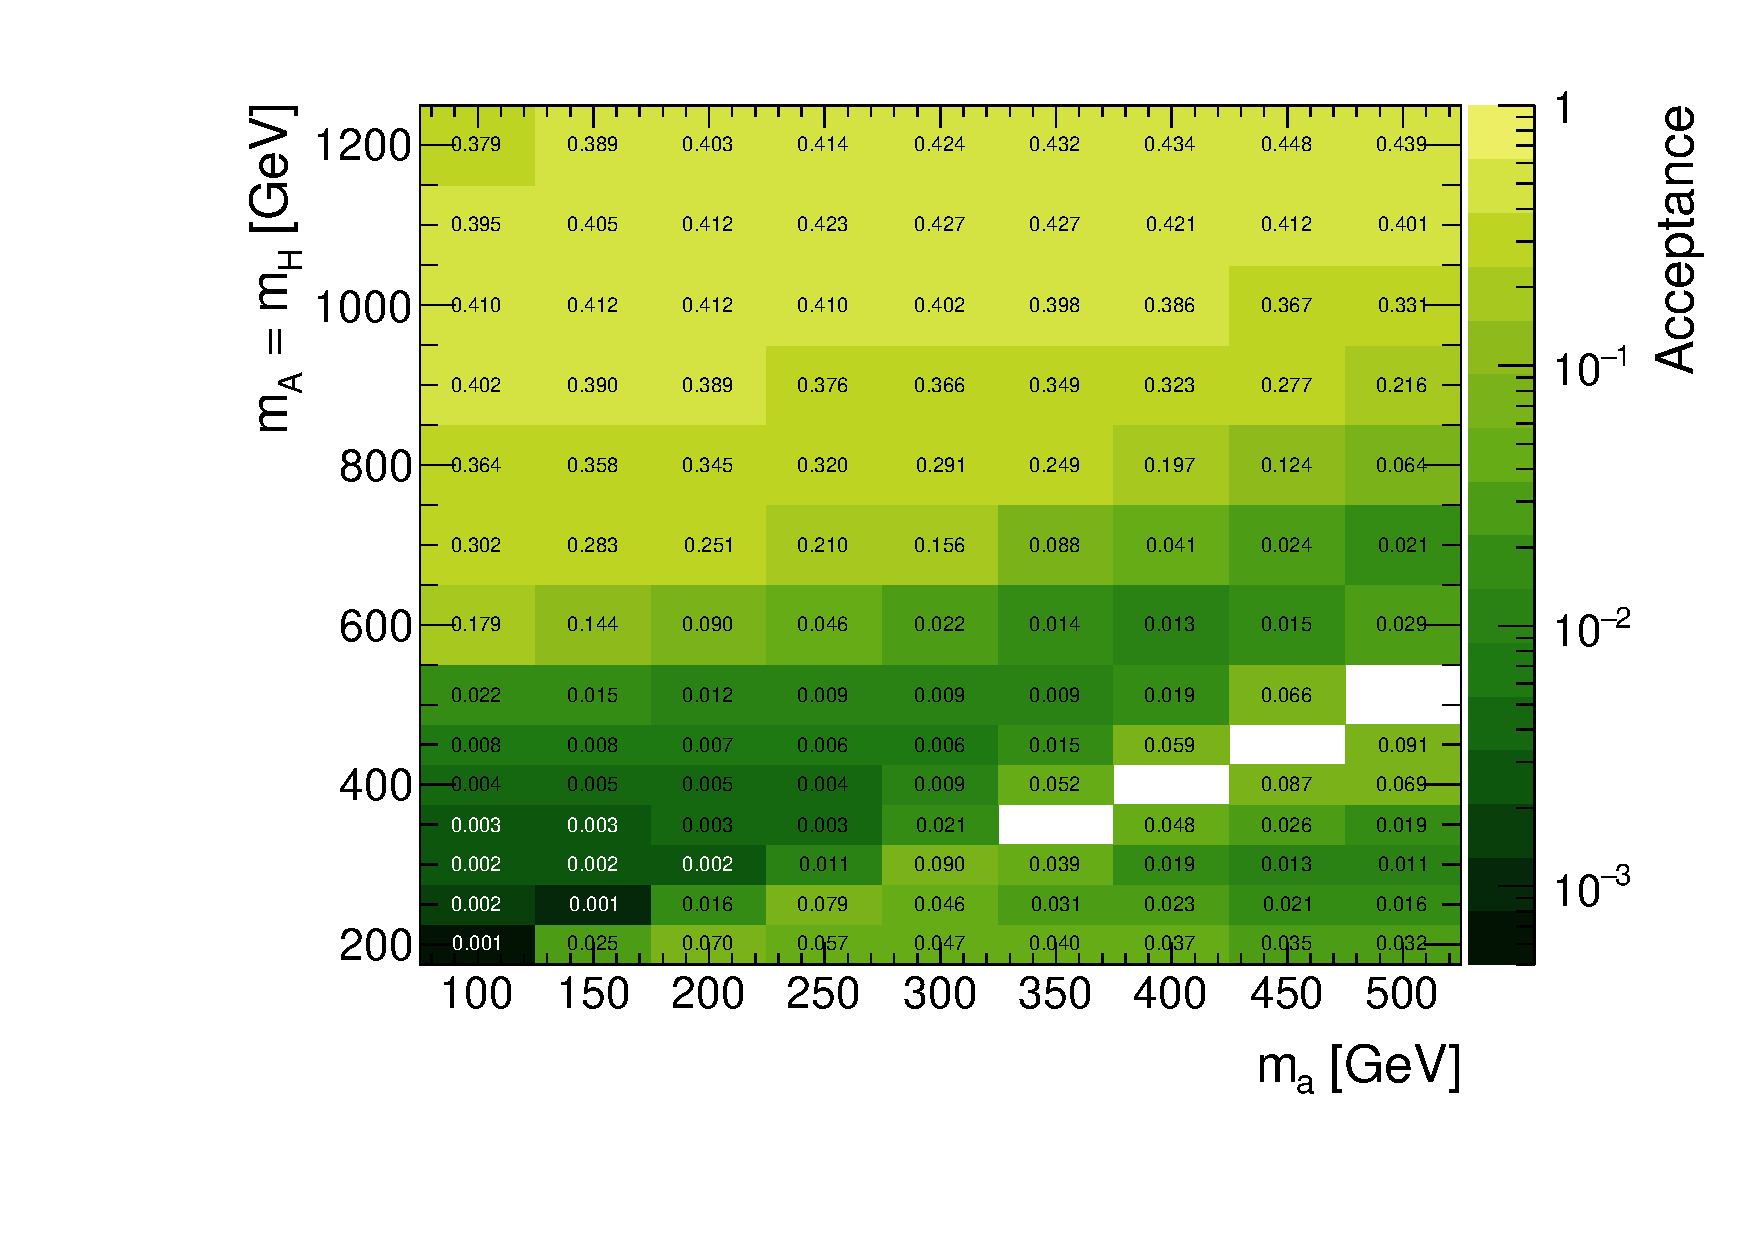
\includegraphics[width=0.45\textwidth]{texinputs/04_grid/figures/monoz/hadronic/grid_mA_ma_merged_acc.pdf}
\caption{Acceptance for the inclusive (top) and final (bottom) selections for the mono-$Z$ hadronic events 
$pp \rightarrow Z(\to q\bar{q})\chi\overline{\chi}$ in the \ma vs \mA grid. Shown on the left (right) is the acceptance for
the resolved (boosted) analysis selections.}
\label{fig:monozhad_acc_ma-mA_grid}
\end{figure}

The signal acceptance for the four sets of event selections given in Table~\ref{tab:monozqq_selection} is 
summarized in Fig.~\ref{fig:monozhad_acc_ma-mA_grid} in the \ma vs \mA grid. Note again that the resolved and boosted 
selection criteria are applied separately for the inclusive case, while for the final selections the boosted criteria are 
applied first and then the resolved ones to those failing the boosted criteria. 
For the inclusive case, the mass dependence on the acceptance is weak for the resolved criteria 
while it is rather significant for the boosted criteria 
as the $Z$-boson is less boosted with decreasing \mA and hence less likely that the $Z$-decay products are merged 
into a single jet. The final boosted selections have acceptance larger than $\sim20$\% (40\%) at 
$\mA>800$ (1000)~GeV and $\ma<400$~GeV. The final resolved selections can recover 10-20\% of signal 
events which fail the boosted criteria in the same mass regions. At $\mA<600$~GeV the signal acceptance 
is dominated by the resolved selection criteria.

\begin{figure}
\centering
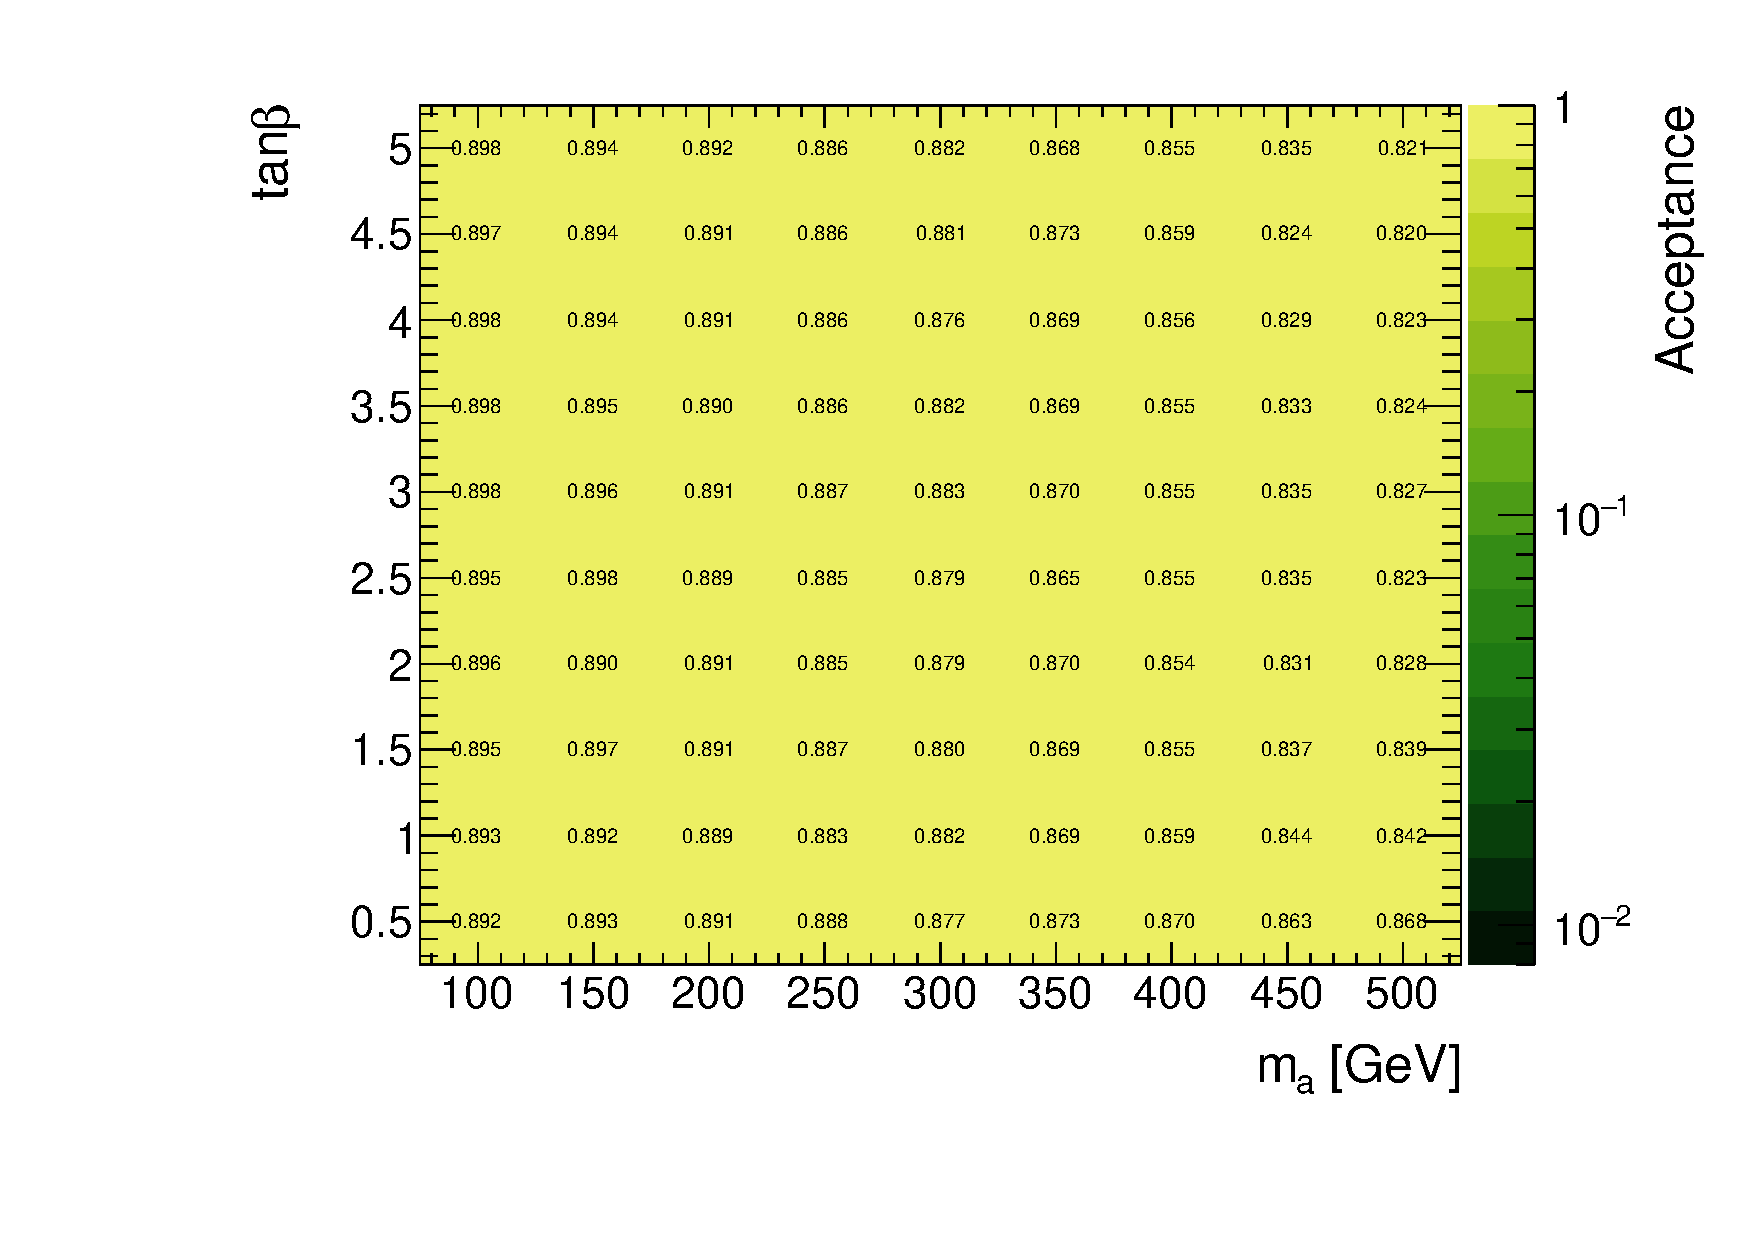
\includegraphics[width=0.45\textwidth]{texinputs/04_grid/figures/monoz/hadronic/grid_tanb_ma_incl_resl_acc.pdf}
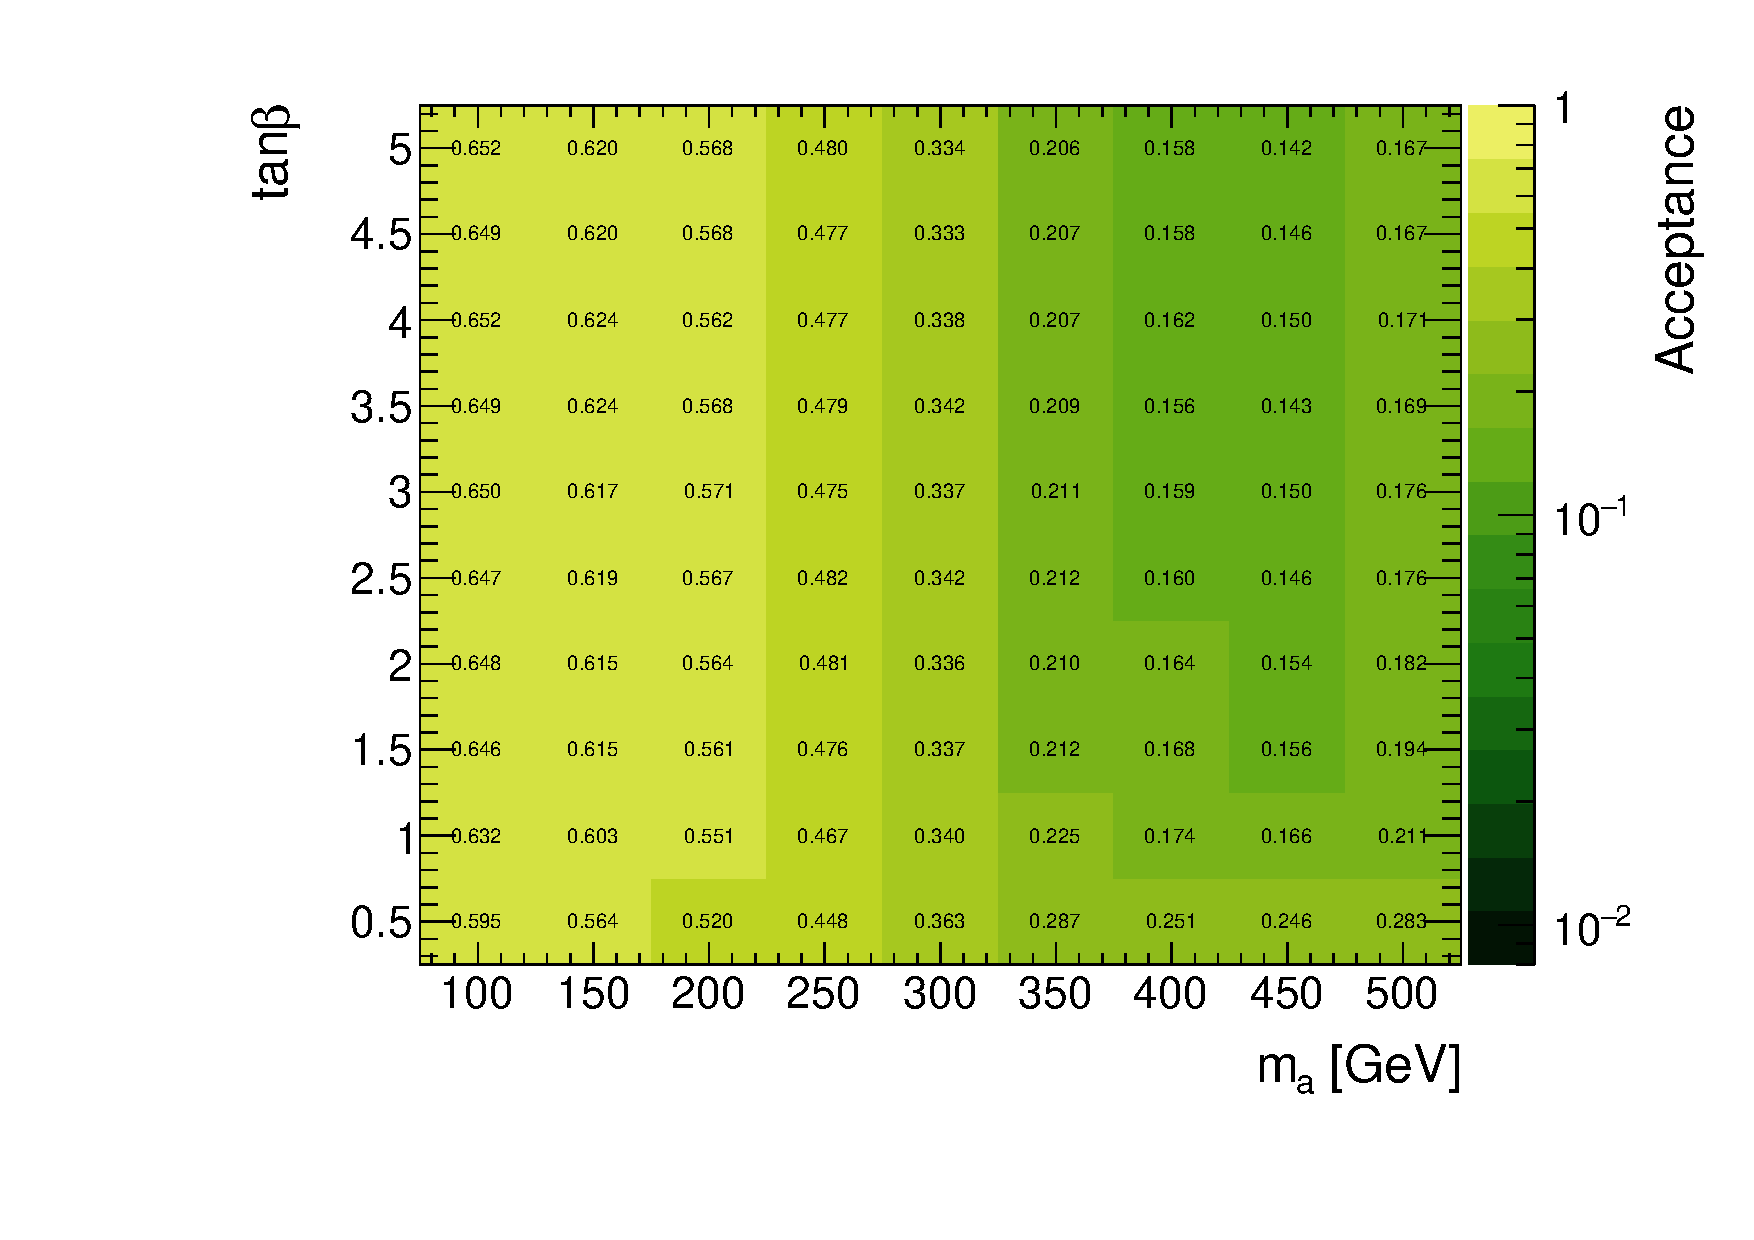
\includegraphics[width=0.45\textwidth]{texinputs/04_grid/figures/monoz/hadronic/grid_tanb_ma_incl_merged_acc.pdf}
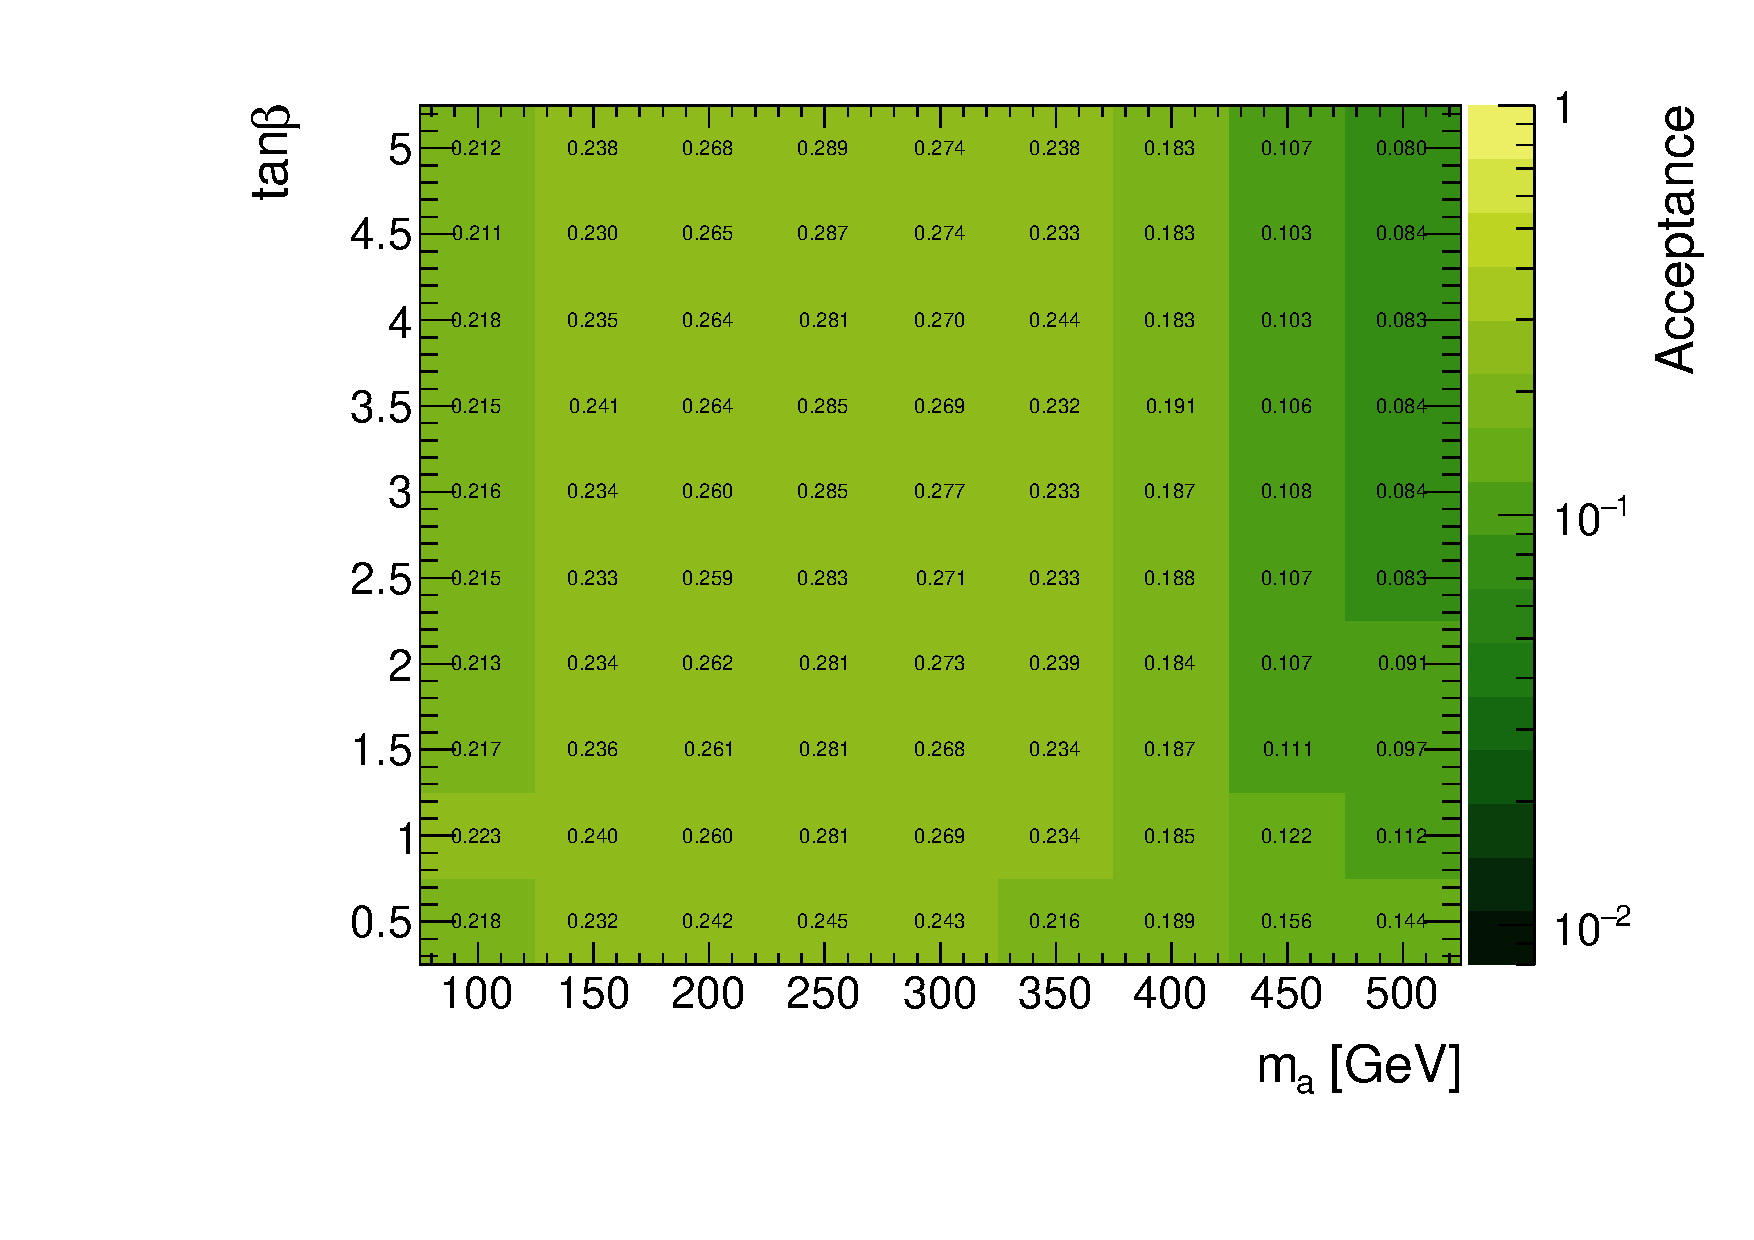
\includegraphics[width=0.45\textwidth]{texinputs/04_grid/figures/monoz/hadronic/grid_tanb_ma_resl_acc.pdf}
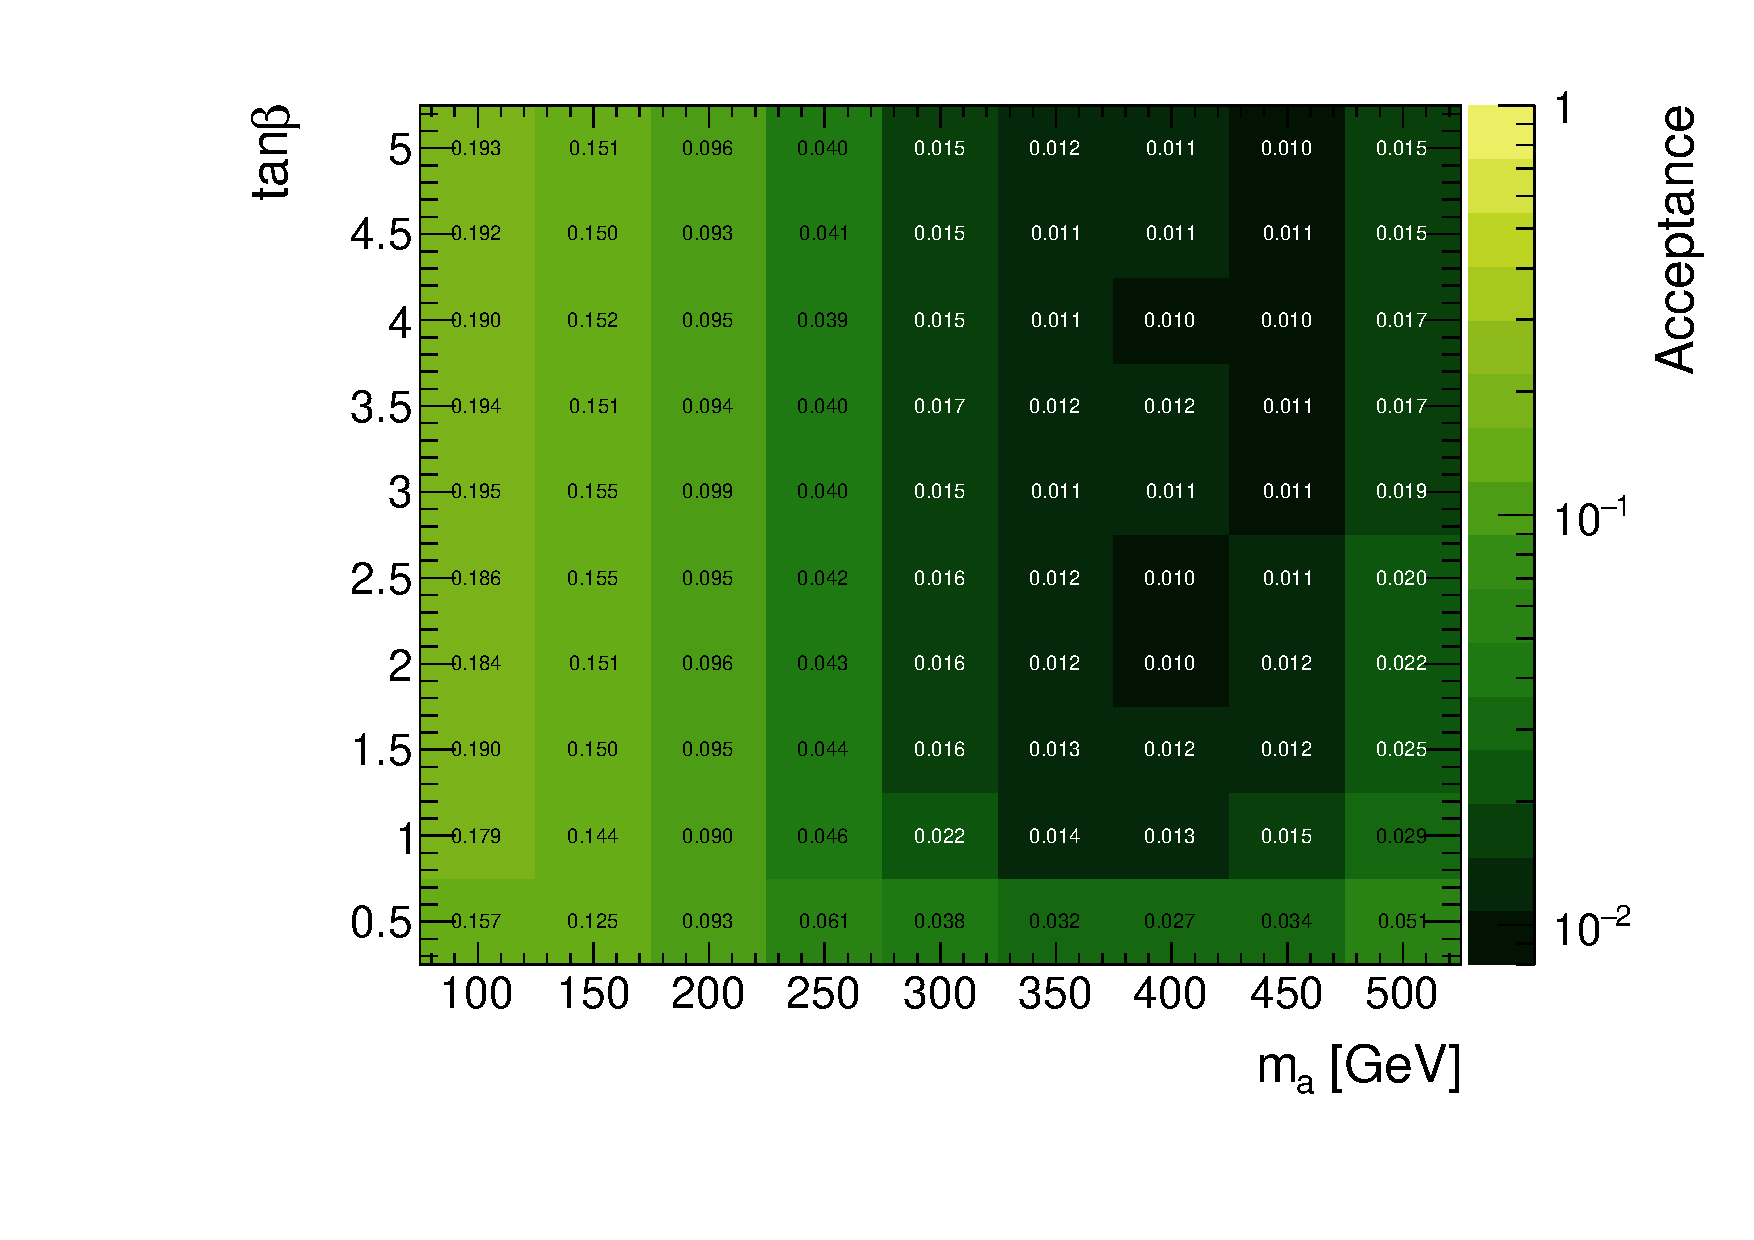
\includegraphics[width=0.45\textwidth]{texinputs/04_grid/figures/monoz/hadronic/grid_tanb_ma_merged_acc.pdf}
\caption{Acceptance for the inclusive (top) and final (bottom) selections for the mono-$Z$ hadronic events 
$pp \rightarrow Z(\to q\bar{q})\chi\overline{\chi}$ in the \ma vs $\tan\beta$ grid. 
Shown on the left (right) is the acceptance for the resolved (boosted) analysis selections. 
The \mA is fixed to 600~GeV.}
\label{fig:monozhad_acc_ma-tanb_grid}
\end{figure}

The signal acceptance in the \ma vs $\tan\beta$ space is shown in Fig.~\ref{fig:monozhad_acc_ma-tanb_grid}. 
The conventions used in Fig.~\ref{fig:monozhad_acc_ma-tanb_grid} are the same as those in 
Fig.~\ref{fig:monozhad_acc_ma-mA_grid}.
The signal acceptance is rather independent of $\tan\beta$ except at low $\tan\beta$ region; the acceptance 
tends to be slightly lower at $\tan\beta<1$ than at $>1$ for $\ma<\sim250$~GeV while it's opposite for 
$\ma>\sim250$~GeV. The acceptance decreases with increasing \ma because the \MET spectrum becomes 
softer with \ma, as shown in Fig.~\ref{fig:monozhad_kin_inc_fixed_mA}.


